\documentclass[]{IEEEtran}

\title{Modellazione e Sintesi di un Moltiplicatore Floating-point Single Precision}
\author{Enrico Sgarbanti - VR446095}

\usepackage{graphicx}
\usepackage{wrapfig}
\usepackage{hyperref}
\usepackage[italian]{babel}
\usepackage[utf8]{inputenc}

\begin{document}
\maketitle



\begin{abstract}
    Questo documento mostra la realizzazione di un moltiplicatore in virgola mobile a precisione singola realizzato in VHDL, Verilog e SystemC ed un componente che permetta di eseguire due moltiplicazioni in parallelo. Il tutto è accompagnato da testbench, sintesi dei componenti VHDL e verilog ed un confronto con l'High-level-Synthesis di un moltiplicatore scritto in c++.
\end{abstract}



\section{Introduzione}
Il progetto consiste nella realizzazione in hardware di un sistema, che attraverso il protocollo di handshake, utilizza due moltiplicatori in virgola mobile a precisione singola, secondo lo standard IEEE754, per eseguire due moltiplicazioni in parello. Esso deve essere sintetizzabile sulla scheda FPGA ``xc7z020clg400-1'' che possedendo solo 125 porte I/O, obbliga a serializzare input e output.
\\Il sistema è stato realizzato in diversi linguaggi al fine di vedere le differenze tra i vari linguaggi utilizzabili per descrivere hardware e capirne i pro e contro. I risultati sono stati poi analizzati e confrontati con quelli ottenuti dall'high level syntesis del codice in c++.
\\L'approccio utilizzato è bottom-up, cioè si è partiti dal moltiplicatore per poi arrivare al top level. L'implementazione è preceduta dall'analisi dei requisiti e dalla stesura della EFSM, cioè la parte più importante in quanto è dove viene tradotto l'algoritmo, descritto il flusso e scelti i vari segnali e registri necessari. Una buona EFSM permette di evitare di scrivere varie righe di codice per poi accorgersi in simulazione che qualcosa non funziona.
\\Ci si aspetta che la versione RTL sia significativamente più performante di quella con l'high level syntesis e che il sistema occupi una minima parte della FPGA in quanto molto piccolo.



\section{Background}

\subsection{Progettazione hardware}
Per la realizzazione di componenti hardware si possono utilizzare diverse tecniche e linguaggi.
\\Un primo approccio è descrivere i componenti a livello RT utilizzando linguaggi di descrizione hardware (\textbf{HDL}) come VHDL e Verilog. Un HDL è un linguaggio specializzato per la descrizione della struttura e del comportamento di circuiti elettronici, in particolare circuiti logici digitali, e la loro analisi e simulazione. Permette inoltre la sintesi di una descrizione HDL in una netlist (una specifica di componenti elettronici fisici e il modo in cui sono collegati insieme), che può quindi essere posizionata e instradata per produrre l'insieme di maschere utilizzate per creare un circuito integrato\cite{HDL}.
\\Un secondo approccio è descrivere le funzionalità del componente con linguaggi più ad alto livello come C, C++ o SystemC\cite{SystemC} e fare High Level Syntesis (\textbf{HLS}) per ottenere una descrizione dell'hardware a livello RT\cite{HLS}.
\\Entrambi gli approcci hanno vantaggi e svantaggi. In particolare HLS riduce i tempi, ma la descrizione hardware generata sarà meno ottimizzata rispetto a quella che si potrebbe ottenere usando un HDL.


\subsection{IEEE 754 single-precision binary floating-point format}
Questo standard definisce il \textbf{formato} per la rappresentazione dei numeri in virgola mobile (compreso $\pm 0$ e i numeri denormalizzati; gli infiniti e i NaN, "not a number"), ed un set di operazioni effettuabili su questi. 
\\In particolare la versione a precisione singola descrive il numero con 32 bit: 1 bit per segno (sign), 8 bit per l'esponente (esp) e 23 bit per la mantissa (mant)\cite{IEEE754}.
\begin{figure}[!htb]
    \centering
    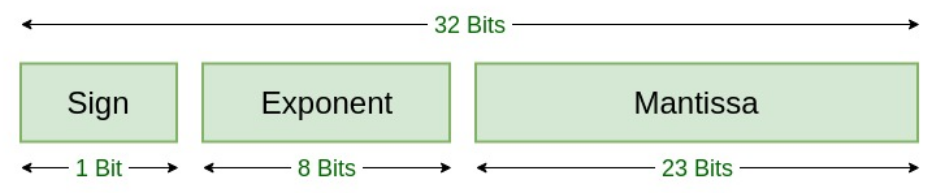
\includegraphics[width=0.9\linewidth]{figures/ieee754_single_precision.png}
    \caption{IEEE 754 single precision}
    \label{fig:IEEE754}
\end{figure}
\\Per la \textbf{codifica} in numero binario:
\begin{itemize}
    \item Dal segno si ricava il bit più significativo (1 se negativato 0 altrimenti).
    \item Si converte il numero in binario.
    \item Si sposta la virgola a sinistra fino ad avere un numero nella forma $1,... \cdot 2^{E}$ dove \textit{E} è il numero di spostamenti.
    \item La mantissa è la parte a destra della virgola, con zeri a destra fino a riempire i 23 bit.
    \item L'esponente esp è uguale a $127+E$ dove 127 è il \textit{bias} di questo standard.
\end{itemize}
Per la \textbf{decodifica} del numero binario: $$(-1)^{sign}\cdot 2^{(esp-127)} \cdot (1 + \sum_{i=1}^{23}b_{23-i}\cdot 2^{-i})$$
\begin{figure}[!htb]
    \centering
    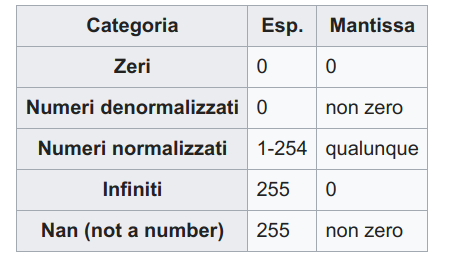
\includegraphics[width=0.6\linewidth]{figures/ieee754_special_case.png}
    \caption{IEEE 754 special case}
    \label{fig:IEEE_SPECIALCASE}
\end{figure}


\subsection{Moltiplicazione di due numeri floating-point}
Qui è riportato un algoritmo utilizzabile per la moltiplicazione fra floating point. Guardare qui per ulteriori dettagli\cite{IEEE754Mult}.
\begin{figure}[!htb]
    \centering
    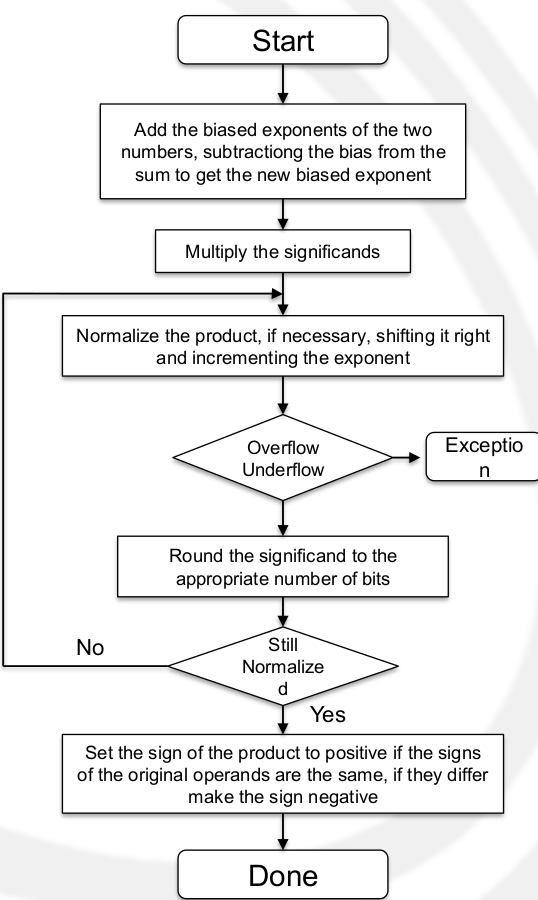
\includegraphics[width=0.6\linewidth]{figures/ieee_multiplication.png}
    \caption{IEEE 754 multiplication}
    \label{fig:IEEE_multiplication}
\end{figure}



\section{Metodologia applicata}

\subsection{Struttura progetto}
\begin{itemize}
    \item \textbf{cpp/}
    \begin{itemize}
        \item \textbf{multiplier.cpp} file dove è presente una funzione che esegue la moltiplicazione in c++.
    \end{itemize}
    \item \textbf{SystemC/} contiene il progetto del sistema scritto interamente in 
    SystemC. La struttura è approfondita qui \ref{section:SystemC}.
    \item \textbf{VHDL\_verilog/}
    \begin{itemize}
        \item \textbf{stimuli/} contiene gli script TCL usati per dei test.
        \item \textbf{waves/} contiene le configurazioni grafiche per visualizzare le simulazioni come negli screenshot.
        \item \textbf{constrains/} contiene i vincoli per la sintesi.
        \item \textbf{double\_multiplier} file Verilog del top level del sistema
        \item \textbf{verilog\_multiplier} file Verilog del moltiplicatore IEEE754
        \item \textbf{vhdl\_multiplier} file VHDL del moltiplicatore VHDL
        \item \textbf{testbench} file Verilog contenente il testbench
    \end{itemize}
\end{itemize}


\subsection{Procedimento}
Il primo passo è stato la realizzazione della EFSM di \textit{multiplier} e \textit{double\_multiplier} che ha portato ad aquisire una visione generale del sistema.
\\Poi si è passati all'implementazione a livello RT con Vivado\cite{Vivado} del \textit{multiplier} in Verilog e VHDL. La loro correttezza è stata testata subito grazie ad uno script TCL osservando gli output a determinati input.
\\Consolidati questi moduli è stato poi possibile realizzare in Verilog il \textit{double\_multiplier} che prende i due componenti e li usa per calcolare due moltiplicazioni. Anch'esso è stato testato con uno script TCL.
\\Completato il sistema è stato fatto un testbench in Verilog per verificare che i moltiplicatori si comportassero allo stesso modo e che reagissero correttamente a casi particolari e numeri arbitrari.
\\In seguito è stato riscritto tutto in SystemC dove si è potuto fare un testbench più fine grazie alla potenza del c++. In particolare sono stati confrontati i valori ottenuti dal sistema con quelli derivati dal risultato convertito in binario della moltiplicazione degli stessi numeri convertiti in float.
\\Infine è stata fatta l'high level syntesis da un semplice codice c++ per confrontare i risultati ottenuti.


\subsection{Vincoli ed Architettura}
Il progetto presenta diversi vincoli:
\begin{itemize}
    \item Il multiplier deve essere scritto in VHDL, verilog e systemC.
    \item Il double\_multiplier deve essere scritto in systemC e un linguaggio a scelta tra VHDL e verilog.
    \item Gli operandi e il risultato devono essere a 32 bit.
    \item I due componenti devono essere sintetizzabili sulla FPGA ``xc7z020clg400-1'' la quale ha a disposizione solo 125 porte.
\end{itemize}
Per far fronte al limite delle porte logiche è stato necessario serializzare input e output. Vengono quindi utilizzati gli stessi 32 bit per il risultato e altri 64 bit per le due coppie di operandi.
\\Grazie al protocollo di \textit{handshake} si sono sincronizzati i vari componenti. Quando il flag \textit{ready} diventa uguale a 1, vengono usati i valori di \textit{op1} e \textit{op2} a quel ciclo di clock per il primo moltiplicatore e quelli del ciclo di clock successivo per il secondo moltiplicatore. Non appena entrambi i moltiplicatori finiranno, il flag \textit{done} del sistema diventerà uguale a 1 e allo stesso ciclo di clock \textit{res} conterrà il risultato della prima moltiplicazione e al ciclo di clock successivo quello della seconda.
\\L'architettura con VHDL e Verilog è mostrata in figura \ref{fig:Architettura}. Quella per SystemC è analoga. 
\\I segnali intermedi sono stati omessi da questa figura, ma vengono descritti nelle sezioni successive.
\begin{figure}[!htb]
    \centering
    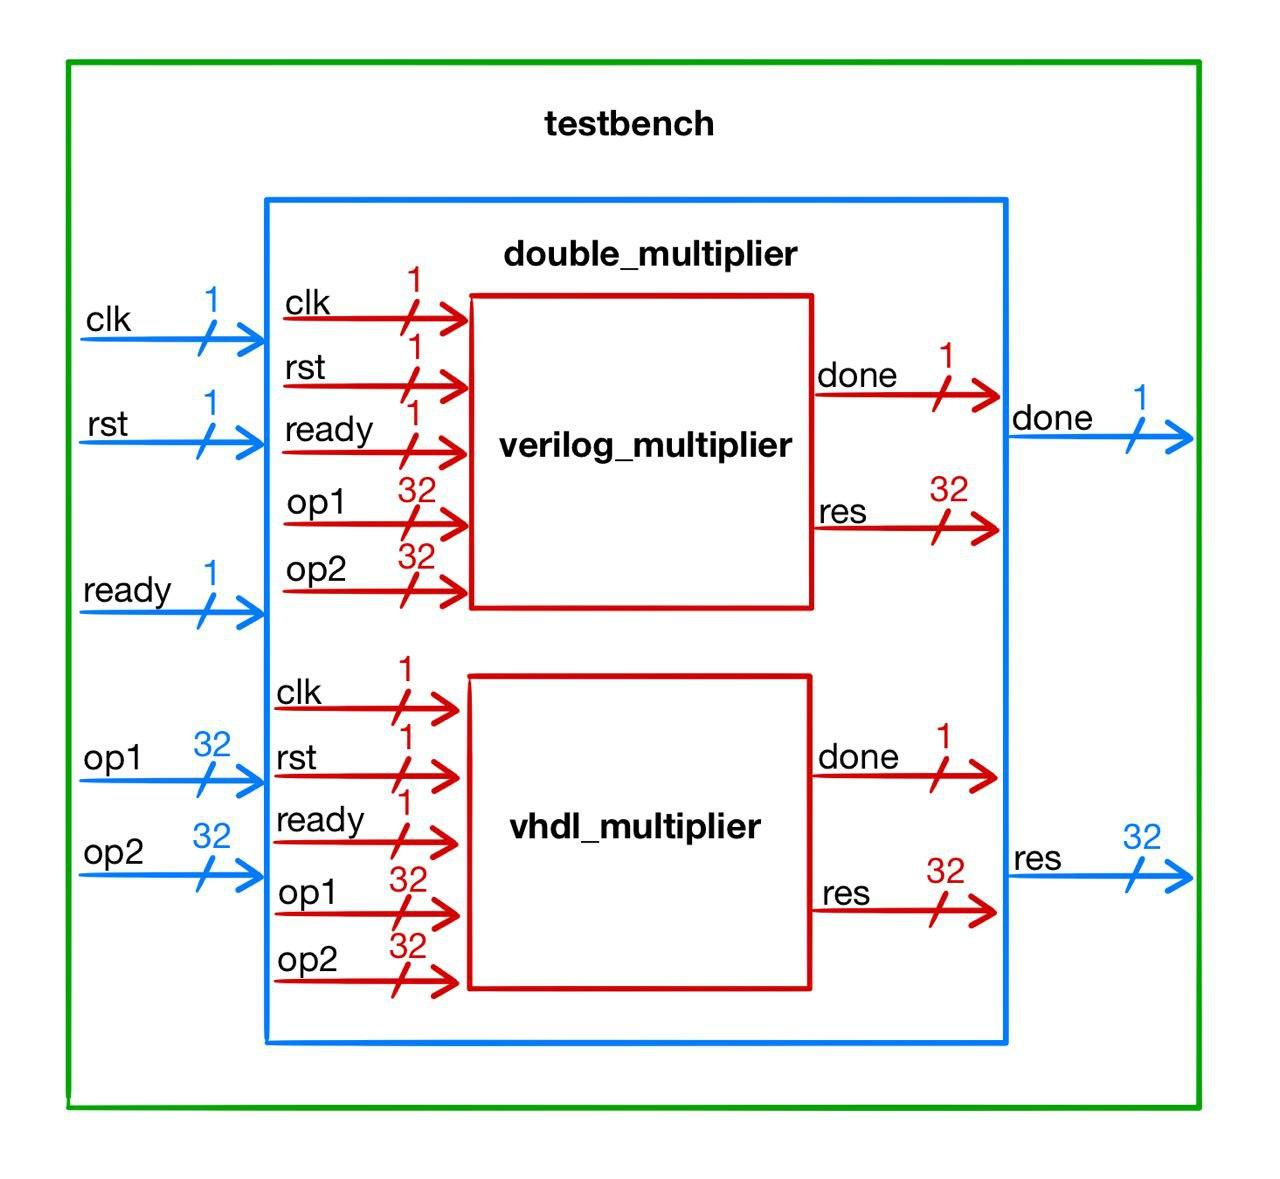
\includegraphics[width=0.8\linewidth]{figures/architettura.jpg}
    \caption{Architettura RTL}
    \label{fig:Architettura}
\end{figure}
La FSMD è realizzata con due processi:
\begin{itemize}
    \item \textbf{fsm:} processo asincrono col compito di calcolare e aggiornare lo stato prossimo.
    \item \textbf{datapath:} processo sincrono che ha il compito di aggiornare lo stato attuale ed elaborare gli output. Esso viene però attivato asincronamente dal fronte di salita del reset al fine di riportare lo stato a quello iniziale.
\end{itemize}


\subsection{multiplier}
Questo componente esegue la moltiplicazione tra numeri floating point a precisione singola. 
\\È stato supposto che gli operandi passati non siano denormalizzati, ma in caso sarebbe facilmente estendibile aggiungendo qualche stato e un segnale di errore in uscita.
\\L'interfaccia è mostrata in figura \ref{fig:Architettura} ed è la stessa per tutte le implementazioni VHDL, Verilog e SystemC: 
\begin{itemize}
    \item \textbf{op1} (32 bit input): primo operando.
    \item \textbf{op2} (32 bit input): secondo operando.
    \item \textbf{clk} (1 bit input): segnale di clock.
    \item \textbf{rst} (1 bit input): segnale di reset. Riporta il sistema allo stato iniziale.
    \item \textbf{ready} (1 bit input): segnale che permette al sistema di uscire dallo stato iniziale. Nello specifico indica che \textit{op1} e \textit{op2} contengono i valori dei due operatori.
    \item \textbf{done} (1 bit output): segnale che indica che il valore su \textit{res} è il risultato.
    \item \textbf{res} (32 bit output): risultato.
\end{itemize}
    
Gli altri segnali/registri intermedi utilizzati sono:
\begin{itemize}
    \item \textbf{norm\_again} (1 bit): indica che la mantissa ha bisogno di essere ulteriormente normalizzata.
    \item \textbf{res\_type} (2 bit): indica il tipo del risultato. Solo nel caso in cui sia un numero si procede all'elaborazione, mentre negli altri casi si passa direttamente allo stato finale.
    \item \textbf{STATE e NEXT\_STATE} (4 bit): rappresentano lo stato attuale e lo stato prossimo.
    \item \textbf{op1\_type e op2\_type} (2 bit): indicano il tipo degli operandi ovvero 0, NaN, $\infty$ oppure un numero.
    \item \textbf{esp\_tmp} (10 bit): permette di eseguire le operazioni per ricavare l'esponente finale senza perdere informazioni.
    \item \textbf{mant\_tmp} (48 bit): permette di eseguire le operazioni per ricavare la mantissa finale senza perdere informazioni.
    \item \textbf{sign1, sign2, esp1, esp2, mant1, mant2}: rappresentano le componenti dei due operandi. \textit{mant1} e \textit{mant2} sono a 24 bit perchè aggiunguno $1.$ alla mantissa che nella rappresentazione IEE754 è omesso.
\end{itemize}

L'algoritmo della moltiplicazione è descritto grazie alla EFSM [Figura \ref{fig:EFSM_MULT}] la quale è formata 14 stati:
\begin{itemize}
    \item \textbf{ST\_START:} stato di partenza. Qui vengono resettati i segnali a zero e inizializzati i registri/variabili contenenti le informazioni di segno, esponente e mantissa degli operanti attuali. In caso di segnale di reset si torna in questo stato. In caso il segnale \textit{ready} vada a 1 si passa a \textit{ST\_EVAL1}.
    \item \textbf{ST\_EVAL1:} qui viene ricavato \textit{op1\_type} cioè se \textit{op1} è 0, $\infty$, NaN o un numero. Poi si passa a \textit{ST\_EVAL2}.
    \item \textbf{ST\_EVAL2:} qui viene ricavato \textit{op2\_type} cioè se \textit{op2} è 0, $\infty$, NaN o un numero. Poi si passa a \textit{ST\_EVAL3}.
    \item \textbf{ST\_EVAL3:} qui viene ricavato \textit{res\_type} cioè se \textit{res} è 0, $\infty$, NaN o un numero. Poi si passa a \textit{ST\_CHECK1}.
    \item \textbf{ST\_CHECK1:} se \textit{res} è un numero si continua con l'elaborazione andando in \textit{ST\_ELAB} altrimenti il risultato è noto e si passa a \textit{ST\_FINISH}. 
    \item \textbf{ST\_ELAB:} qui si ricava l'esponente temporaneo di \textit{res} sommando gli esponenti degli operandi e sottraendo il bias. Esso è a 10bit anzichè 8bit per permettere di compiere l'operazione senza perdere informazioni. Viene ricavato anche la mantissa temporanea che sarà di 48bit per contenere la moltiplicazione delle mantesse dei due operandi. Poi si passa a \textit{ST\_UNDERF}.
    \item \textbf{ST\_UNDERF:} qui si controlla se il bit più significativo di \textit{esp\_tmp} è 1. Essendo codificato in complemento a 2, il fatto che sia 1 implica che è un numero negativo e quindi si è verificato un underflow e \textit{res\_type} sarà 0.
    \item \textbf{ST\_CHECK2:} se \textit{res} non è zero si continua con l'elaborazione andando in \textit{ST\_NORM1} altrimenti il risultato è noto e si passa a \textit{ST\_FINISH}. 
    \item \textbf{ST\_NORM1:} qui si effettua la normalizzazione della mantissa. Se il bit più significativo è 1 allora vuol dire la mantissa ha due cifre a sinistra della virgola e quindi deve essere normalizzata cioè riporta alla forma in cui c'è solo un 1 a sinistra. Per normalizzare basta incrementare l'esponente e considera la virgola spostata a sinistra. Nel caso in cui il bit più significativo sia 0 si fa uno shift a sinistra al fine di avere la virgola a destra del bit più significativo. Poi si passa a \textit{ST\_ROUND}.
    \item \textbf{ST\_ROUND:} qui si controlla se c'è bisogno di arrotondare la mantissa, che da 48bit dovrà passare a 23bit, e in caso affermativo si pone a 1 \textit{norm\_again}. Si è deciso di arrotondare solo se il 23esimo bit, cioè quello a destra del punto di taglio, vale 1. Poi si passa a \textit{ST\_CHECK3}.
    \item \textbf{ST\_CHECK3:} se \textit{norm\_again} vale 1 si passa a \textit{ST\_NORM2} altrimenti a \textit{ST\_OVERF}. 
    \item \textbf{ST\_NORM2:} qui avviene l'incremento della mantissa a causa dell'arrotondamento. Nel caso in cui la mantissa fosse formata da tutti 1 l'incremento la riporterebbe a tutti 0 e l'esponente andrebbe incrementato. Poi si passa a \textit{ST\_OVERF}.
    \item \textbf{ST\_OVERF:} qui avviene il controllo dell'overflow guardando se il secondo bit più significativo di \textit{esp\_tmp} vale 1 e in caso affermativo \textit{res\_type} sarà $\infty$. Infine si passa a \textit{ST\_FINISH}.
    \item \textbf{ST\_FINISH:} qui si ricava il segno del risultato facendo lo XOR fra quello degli operandi, mentre si ricava il resto in base al valore di \textit{res\_type}. Infine si imposta \textit{done} a 1 e si torna in \textit{ST\_START}.
\end{itemize}


\subsection{double\_multiplier}
Questo componente esegue due moltiplicazioni tra numeri floating point a precisione singola.
\\La scelta di realizzarlo in Verilog è stata del tutto arbitraria.
\\L'interfaccia è mostrata in figura \ref{fig:Architettura} ed è la stessa sia per l'implementazione Verilog che quella SystemC:
\begin{itemize}
    \item \textbf{op1} (32 bit input): primo operando.
    \item \textbf{op2} (32 bit input): secondo operando.
    \item \textbf{clk} (1 bit input): segnale di clock.
    \item \textbf{rst} (1 bit input): segnale di reset. Riporta il sistema allo stato iniziale.
    \item \textbf{ready} (1 bit input): segnale che permette al sistema di uscire dallo stato iniziale. Nello specifico indica che in questo ciclo di clok \textit{op1} e \textit{op2} contengono gli operandi della prima moltiplicazione e nel ciclo di clock successivo ci saranno quelli per la seconda moltiplicazione.
    \item \textbf{done} (1 bit output): segnale che indica che il valore su \textit{res} è il risultato.
    \item \textbf{res} (32 bit output): risultato.
\end{itemize}
    
Gli altri segnali/registri intermedi utilizzati sono:
\begin{itemize}
    \item \textbf{ready1} (1 bit) segnale che pone il \textit{ready} del primo multiplier (quello in Verilog) a 1.
    \item \textbf{ready2} (1 bit) segnale che pone il \textit{ready} del secondo multiplier (quello in VHDL) a 1.
    \item \textbf{done1} (1 bit) segnale che indica che il valore su \textit{res1} è il risultato della prima moltiplicazione.
    \item \textbf{done2} (1 bit) segnale che indica che il valore su \textit{res2} è il risultato della seconda moltiplicazione.
    \item \textbf{op1\_tmp, op2\_tmp} (32 bit) che servono a memorizzare temporaneamente gli operandi per la prima moltiplicazione.
\end{itemize}

L'algoritmo è descritto grazie alla EFSM [Figura \ref{fig:EFSM_DM}] la quale è formata 8 stati:
\begin{itemize}
    \item \textbf{ST\_START:} pone \textit{done}, \textit{ready1} e \textit{ready2} uguali a 0 e inizializza \textit{op1\_tmp1} e \textit{op2\_tmp1} rispettivamenete con i valori di \textit{op1} e \textit{op2} i quali serviranno per il primo moltiplicatore. Si rimane qui finchè \textit{ready} vale 0 altrimensi si passa a \textit{ST\_RUN1}. Se in qualsiasi stato si riceve \textit{reset} uguale a 1 allora si passa a questo stato e si pone \textit{rst} uguale a 1 entrambi i \textit{rst} dei multiplier.
    \item \textbf{ST\_RUN1:} pone \textit{ready1} uguale a 1, attivando quindi il primo moltiplicatore, e inizializza \textit{op1\_tmp2} e \textit{op2\_tmp2} rispettivamenete con i valori di \textit{op1} e \textit{op2} i quali serviranno per il secondo moltiplicatore.
    \item \textbf{ST\_RUN2:} pone \textit{ready1} uguale a 0 e \textit{ready2} uguale a 1, attivando quindi il secondo moltiplicatore.
    \item \textbf{ST\_WAIT:} pone \textit{ready2} uguale a 0. Si rimane in questo stato finchè \textit{done1} $=1$ e in quel caso si passa a \textit{ST\_WAIT2} oppure che \textit{done2} $=1$ passando a {ST\_WAIT1}. Nel caso in cui sia \textit{done1} $=1$ che \textit{done2} $=1$ allora si passa direttamente a \textit{ST\_RET1}.
    \item \textbf{ST\_WAIT1:} si resta qui finchè non finisce anche il primo moltiplicatore, cioè finchè \textit{ready1} $=0$.
    \item \textbf{ST\_WAIT2:} si resta qui finchè non finisce anche il secondo moltiplicatore, cioè finchè \textit{ready2} $=0$.
    \item \textbf{ST\_RET1:} pone \textit{done} uguale a 1 e \textit{res} uguale al risultato del primo moltiplicatore cioè \textit{res1}.
    \item \textbf{ST\_RET2:} pone \textit{res} uguale al risultato del secondo moltiplicatore cioè \textit{res2} e ritorna allo stato iniziale.
\end{itemize}


\subsection{Implementazione RTL con Verilog e VHDL}
In \textbf{verilog\_multiplier} e \textit{double\_multiplier}
\begin{itemize}
    \item Sono definiti come ``wire'' tutti i segnali collegati alle porte di input mentre come ``reg'' tutti i registri collegati alle porte di output e quelli intermedi.
    \item Gli stati e \textit{op1\_type, op2\_type, res\_type} sono stati definiti come ``parameter''.
\end{itemize}
In \textbf{vhdl\_multiplier:}
\begin{itemize}
    \item Sono usate le librerie ``IEEE.STD\_LOGIC\_1164.ALL'' per abilitare i tipi std\_logic e ``use IEEE.NUMERIC\_STD.ALL'' per usare funzioni aritmetiche con valori signed e unsigned
    \item Sono definiti come ``signal'' tutti i segnali collegati alle porte di input e output.
    \item Sono definiti come ``signal'' tutti i segnali interni di communicazione per la FSM.
    \item Sono definite come ``variable'' \textit{sign1, sign2, esp1, esp2, esp\_tmp, mant1, mant2, mant\_tmp, op1\_type, op2\_type} perchè utilizzati solo all'interno del processo ``datapath''.
    \item Gli stati e \textit{op1\_type, op2\_type, res\_type} sono stati definiti all'interno del \textit{package} rispettivamente come ``MULT\_STATE'' e ``MULT\_TYPE''.
    \item L'architettura utilizzata segue lo stile ``behavioral'', cioè quello più ``program-like'' in quanto più semplice e chiaro per descrivere una FSMD con due processi.
\end{itemize}


\subsection{Implementazione RTL con SystemC \label{section:SystemC}}
Si creano i seguenti files e directory:
\begin{itemize}
    \item \textbf{Makefile:} tool per la compilazione automatica del progetto. Richiede che la variabile d'ambiente SYSTEMC\_HOME contenga il path alla libreria di SystemC.
    \item \textbf{bin:} directory che contiene l'eseguibile \textit{double\_multiplier\_RLT.x} (generato dopo la compilazione) e \textit{wave.vcd} (generato dopo l'esecuzione dell'eseguibile).
    \item \textbf{obj:} directory che contiene i files oggetto (generati dopo la compilazione)
    \item \textbf{include:} directory che contiene gli headers \textit{double\_multiplier\_RTL.hh}, \textit{multiplier\_RTL.hh}, \textit{testbench\_RTL.hh}. Qui sono definite tutte le porte, segnali, variabili ed enumerazioni dei vari componenti
    \item \textbf{src:} directory che contiene i files sorgenti \textit{double\_multiplier\_RTL.cc}, \textit{multiplier\_RTL.cc}, \textit{testbench\_RTL.cc} e \textit{main\_RTL.cc}.
\end{itemize}
In \textbf{double\_multiplier\_RTL.hh}
\begin{itemize}
    \item Sono definiti come ``sc\_signal'' tutti i segnali collegati alle porte di input e output.
    \item Sono definiti come ``sc\_signal'' tutti i segnali interni di communicazione per la FSM.
    \item Gli stati sono stati definiti come ``enumerazioni''.
\end{itemize}
In \textbf{multiplier\_RTL.hh}
\begin{itemize}
    \item Sono definiti come ``sc\_signal'' tutti i segnali collegati alle porte di input e output.
    \item Sono definiti come ``sc\_signal'' tutti i segnali interni di communicazione per la FSM.
    \item Sono definite come variabili di SystemC \textit{sign1, sign2, esp1, esp2, esp\_tmp, mant1, mant2, mant\_tmp, op1\_type, op2\_type} perchè utilizzati solo all'interno del processo ``datapath''.
    \item Gli stati e \textit{op1\_type, op2\_type, res\_type} sono stati definiti come ``enumerazioni''.
\end{itemize}
A differenza di verilog e VHDL, in SystemC è necessario un file ``main'' che contenga il metodo \textit{sc\_main} e che permetta di collegare il componente da testare con il testbench. In esso si utilizza \textit{sc\_create\_vcd\_trace\_file} per salvare le tracce necessarie a lanciare una simulazione con tools come gtkwave.
\\Per eseguire il componente bisogna usare i comandi:
\begin{itemize}
    \item \textbf{make: } per compilare.
    \item \textbf{./bin/double\_multiplier\_RTL.x:} per eseguire il programma.
    \item \textbf{gtkwave/wave.vcd:} per lanciare la simulazione.
\end{itemize}



\section{Testbench}
Il \textbf{testbench in Verilog}, [Figura ref{fig:SIM1}], aspetta un po di tempo, perchè altrimenti si verificherebbero problemi dovuti allo startup della FPGA nella simulazione post-sintesi, e poi esegue due volte il \textit{double\_multiplier}, prima con due coppie di operandi che danno come risultato dei numeri normali, e poi con due coppie di operandi che danno come risultati dei casi speciali. \\\\


Il \textbf{testbench in SystemC} mette a disposizione tre thread da attivare togliendo i commenti nel costruttore del ``TestbenchModule'':
\begin{itemize}
    \item \textbf{targeted\_test:} test analogo a quello in Verilog. [Figura ref{fig:SIM2}].
    \item \textbf{rnd\_test:} test che prova \textit{TESTS\_NUM} moltiplicazioni generate casualmente tra un intervallo modificabile. [Figura ref{fig:SIM3}].
    \item \textbf{run\_all:} che prova tutte le possibili combinazioni cioè \(2^{32} * 2^{32}\). Si può limitare il numero di combinazioni evitando di contare il bit del segno, in quanto il calcolo è un semplice xor. Poi si possono escludere tutti i numeri denormalizzati. In ogni caso risulta troppo pesante per essere eseguito.
\end{itemize}



\section{risultati}

\subsection{Simulazioni con script TCL}
% Per testare il corretto funzionamento dei componenti è stata fatta la simulazione con gli script in figura ref{fig:SCRIPT_MULT} e figura ref{fig:SCRIPT_DOUBLE}. Lo scopo di questi test è verificare il corretto funzionamento dei componenti avendo a disposizione tutti i segnali interni e stati.
% \\In particolare modificando il codice sono stati controllati casi particolari come la reazione del sistema al variare inaspettato degli operandi o di \textit{ready}, operazioni con operatori speciali e il comportamento con la richiesta di una nuova elaborazione.
% \\Un altro controllo fatto è il verificare che l'esecuzione del multiplier Verilog sia analoga a quella del multiplier VHDL.
% \\Le varie simulazioni sono riportate nelle figure \ref{fig:SIM_MULT_VERILOG} \ref{fig:SIM_MULT_VHDL} \ref{fig:SIM_DM}.

\subsection{Simulazione con testbench in Verilog}
I test precedenti servivano ad assistere la progettazione, questo invece a verificare la correttezza del sistema. Sono infatti testati tutti i casi particolari e valori scelti arbitrariamente.














\section{Conclusioni}


\bibliographystyle{IEEEtran}
\bibliography{biblio}
\appendix

\begin{figure*}[bt]
    \centering
    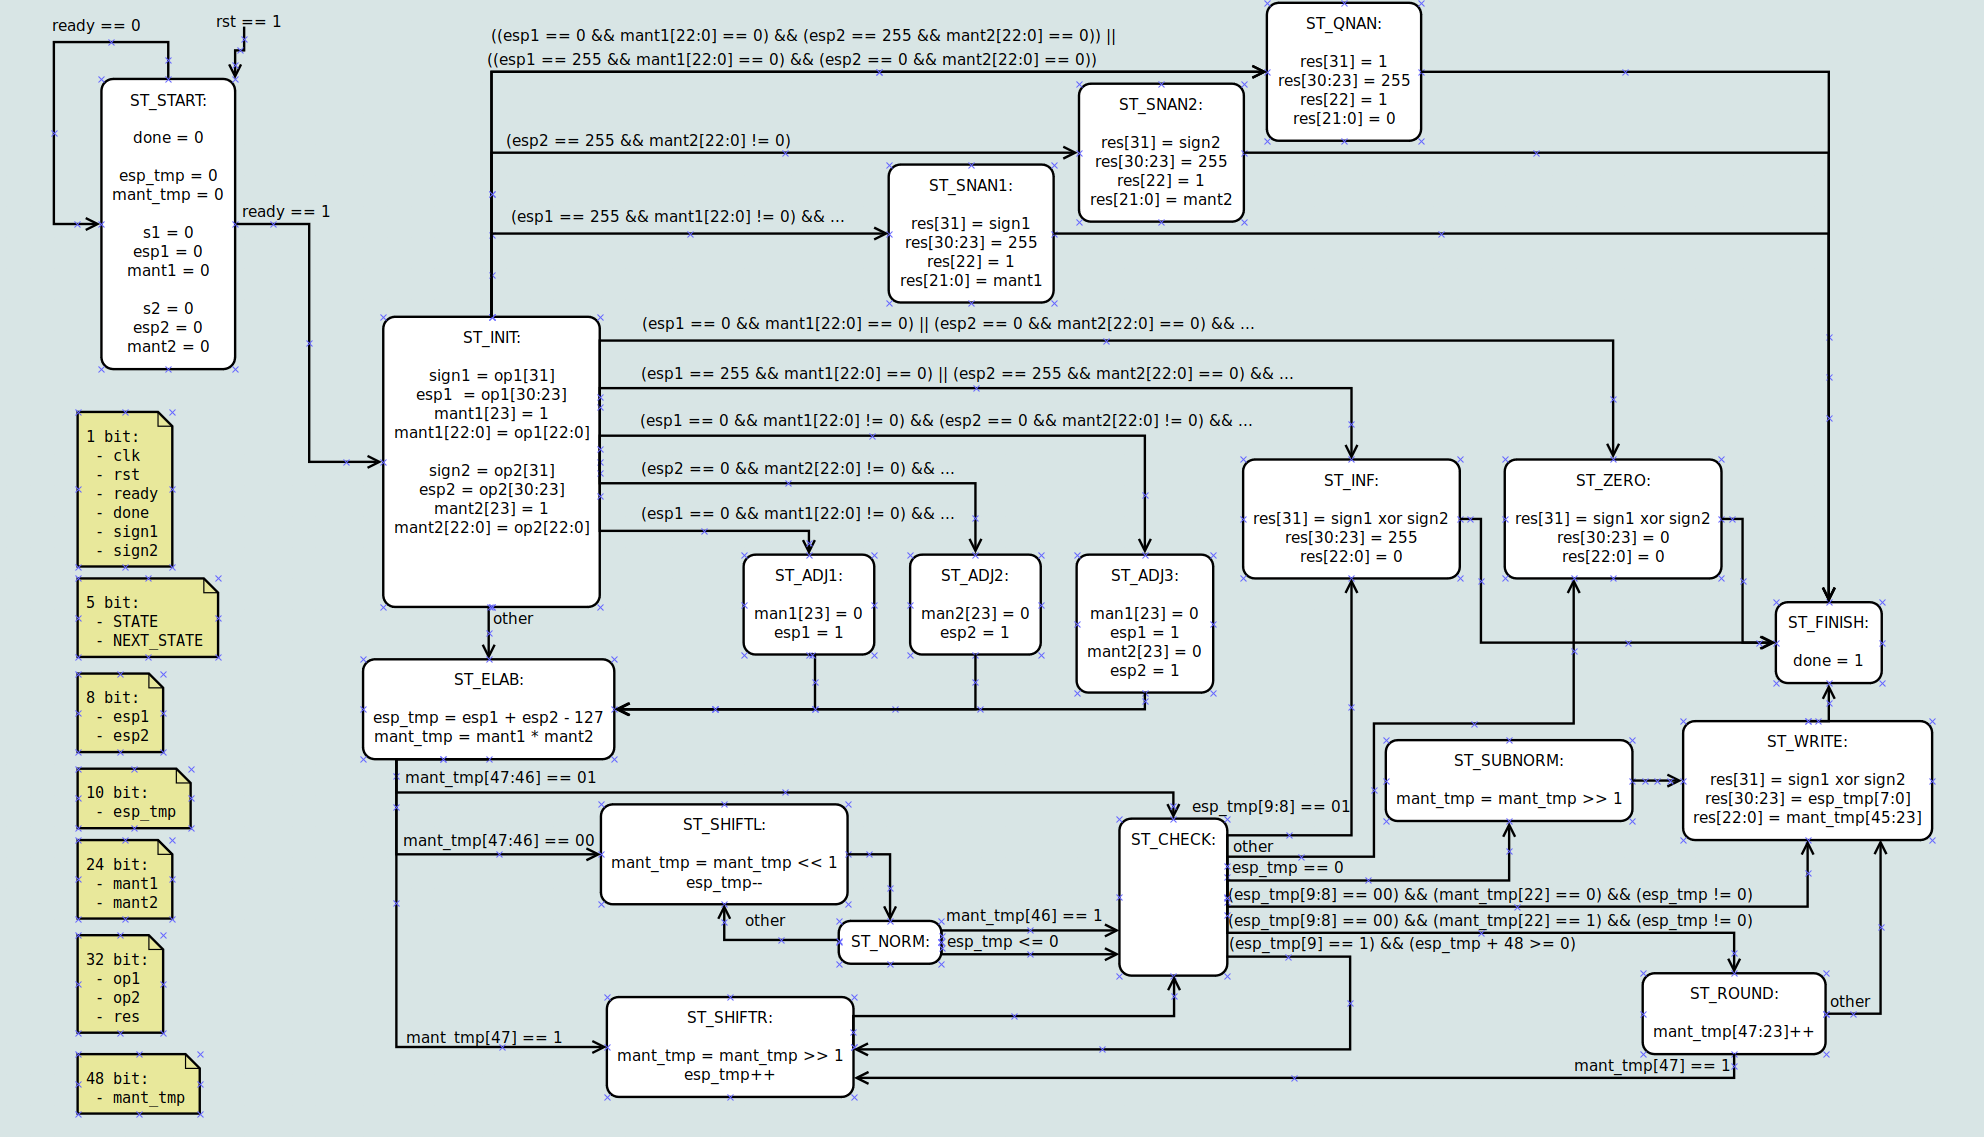
\includegraphics[width=\textwidth]{figures/EFSM_mult}
    \caption{EFSM del multiplier}
    \label{fig:EFSM_MULT}
\end{figure*}

\begin{figure*}[bt]
    \centering
    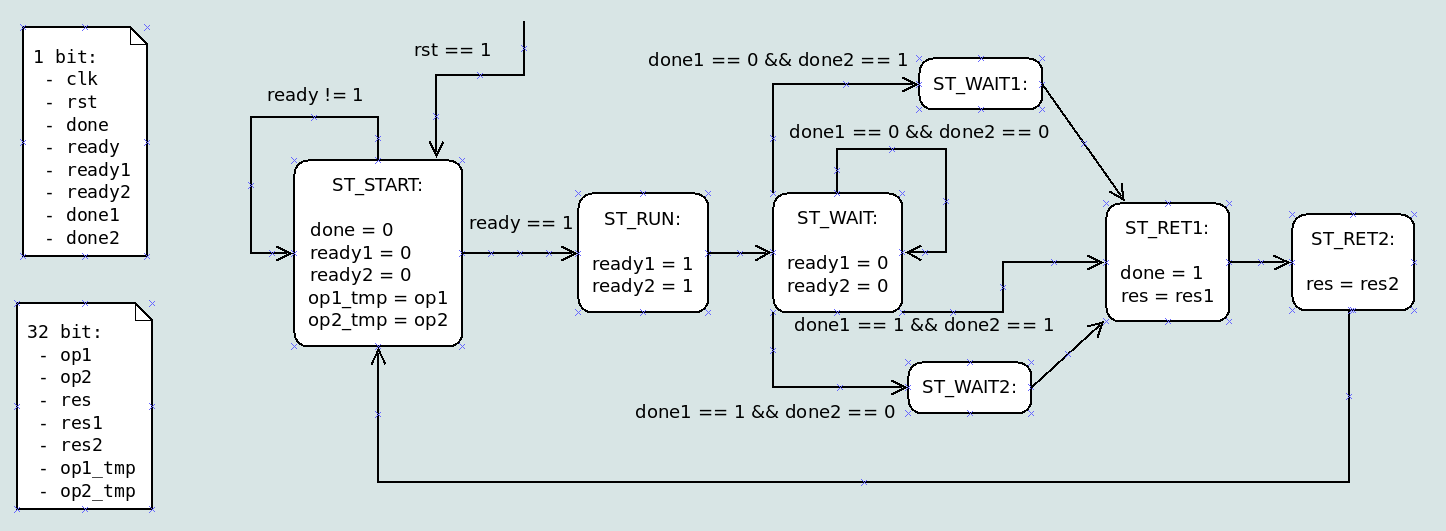
\includegraphics[width=\textwidth]{figures/EFSM_dm}
    \caption{EFSM del double\_multiplier}
    \label{fig:EFSM_DM}
\end{figure*}

\begin{figure*}[bt]
    \centering
    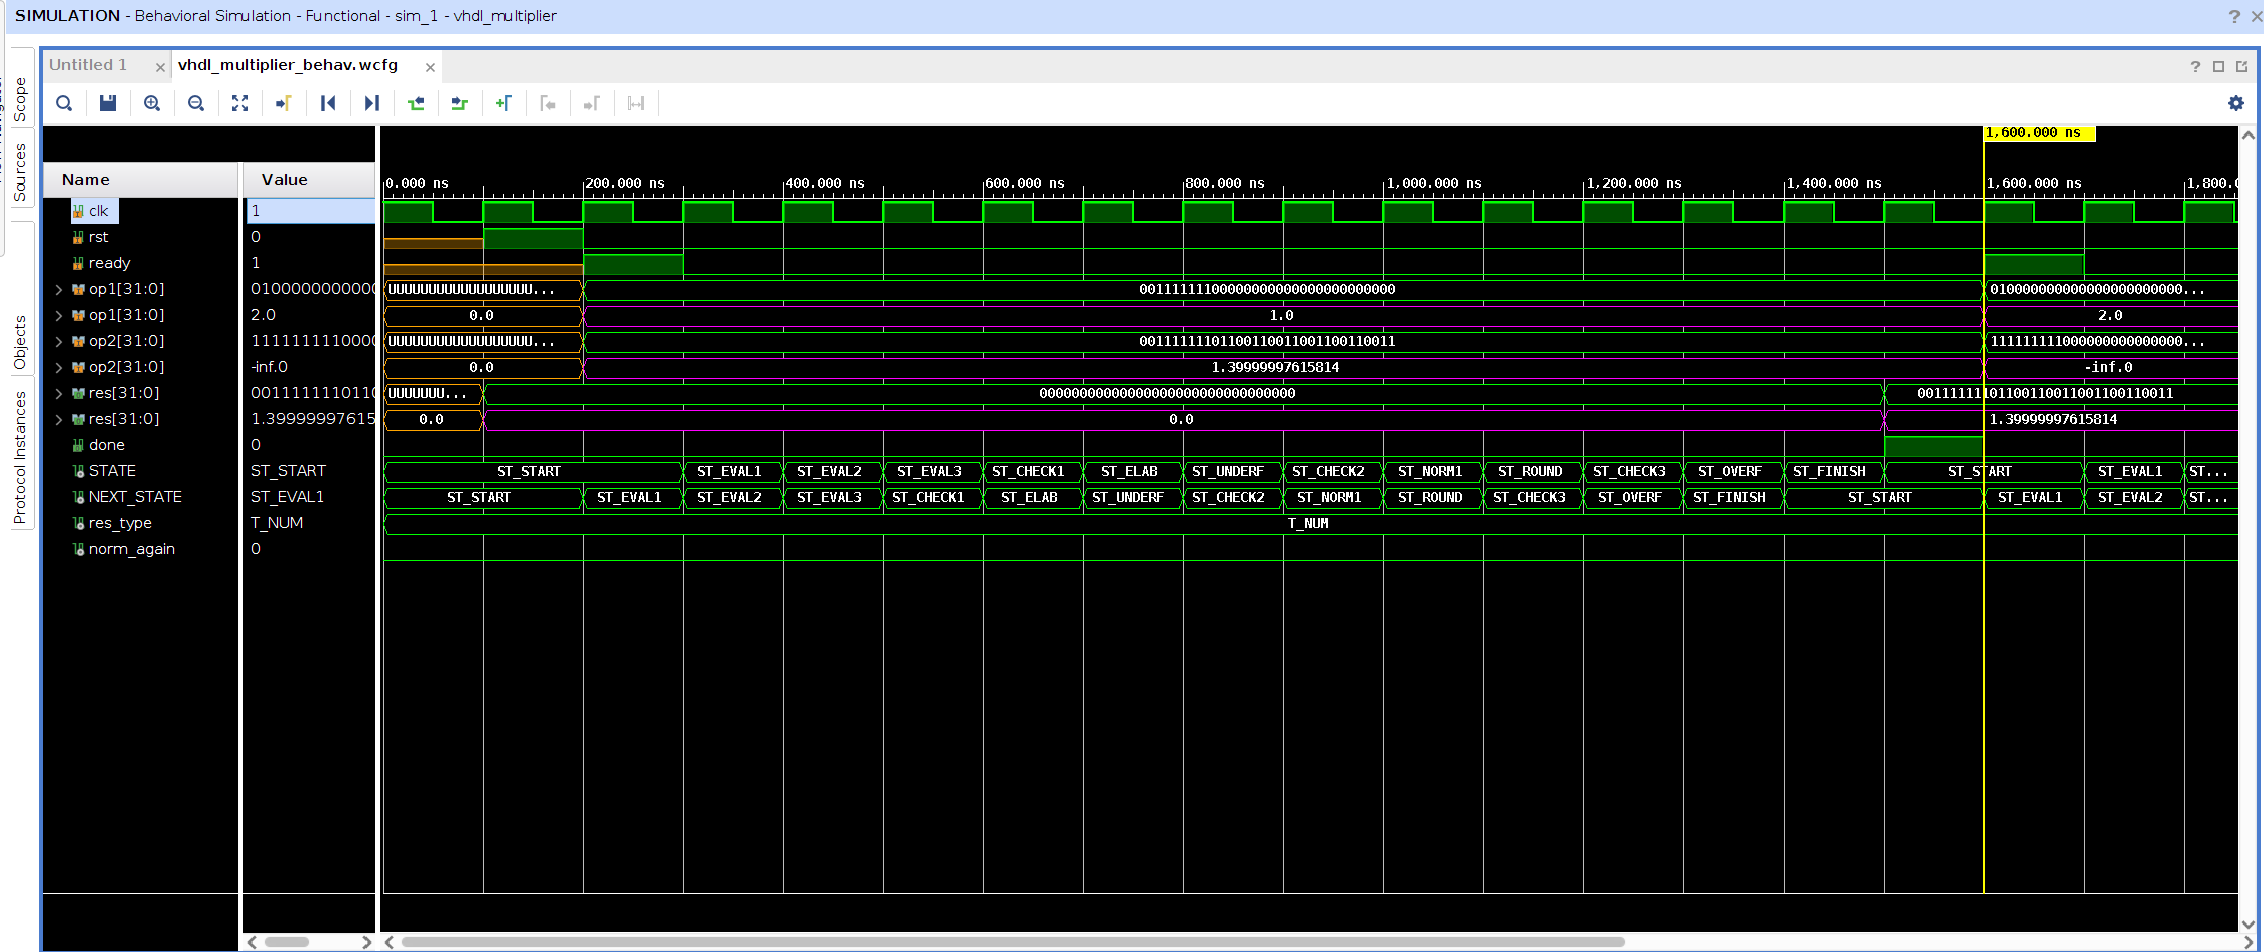
\includegraphics[width=\textwidth]{figures/sim_mult_vhdl_zoom}
    \caption{Simulazione multiplier in VHDL con script TCL con più zoom}
    \label{fig:SIM_MULT_VHDL_ZOOM}
\end{figure*}

\begin{figure*}[bt]
    \centering
    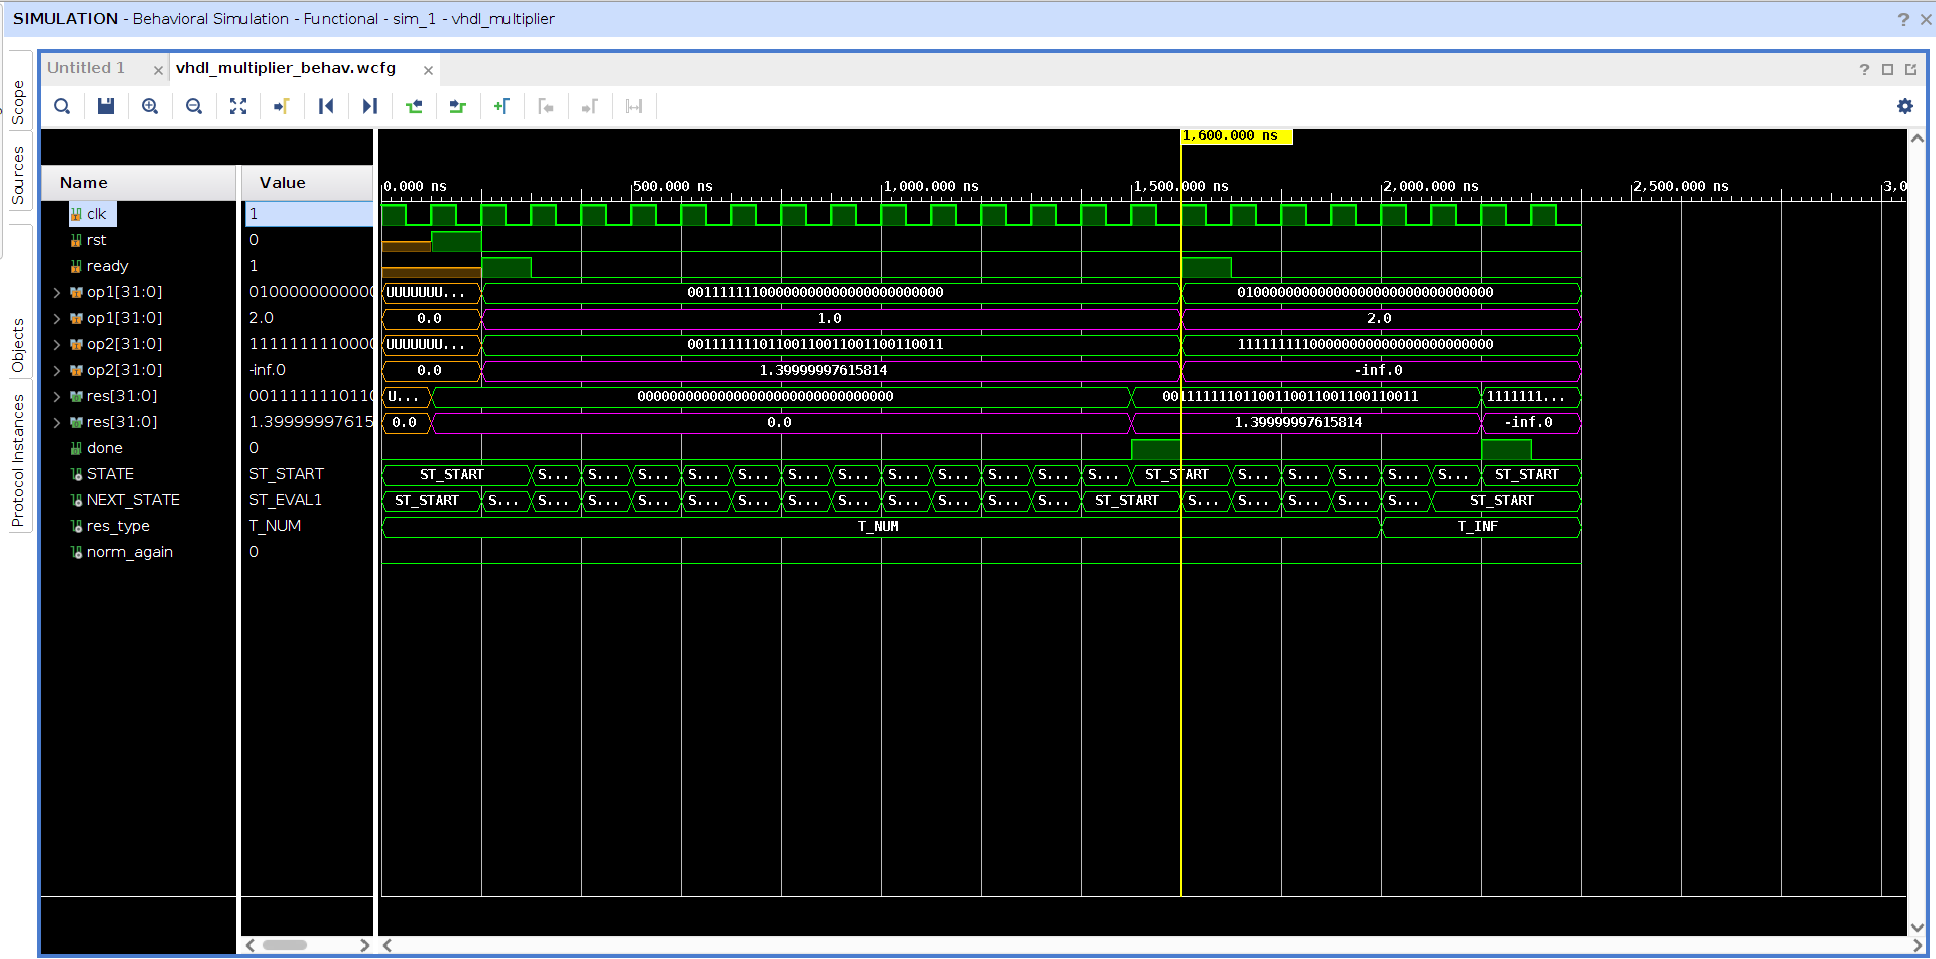
\includegraphics[width=\textwidth]{figures/sim_mult_vhdl}
    \caption{Simulazione multiplier in VHDL con script TCL}
    \label{fig:SIM_MULT_VHDL}
\end{figure*}

\begin{figure*}[bt]
    \centering
    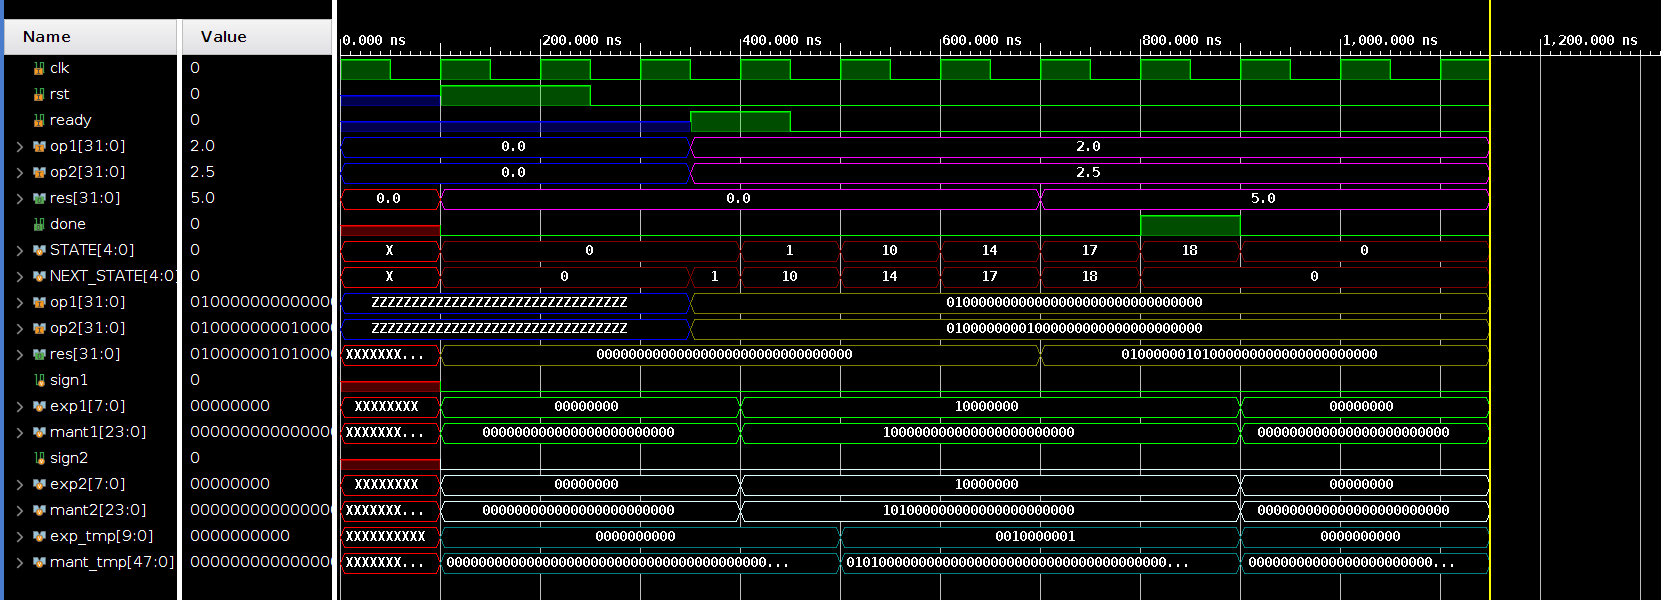
\includegraphics[width=\textwidth]{figures/sim_mult_verilog}
    \caption{Simulazione multiplier in Verilog con script TCL}
    \label{fig:SIM_MULT_VERILOG}
\end{figure*}

\begin{figure*}[bt]
    \centering
    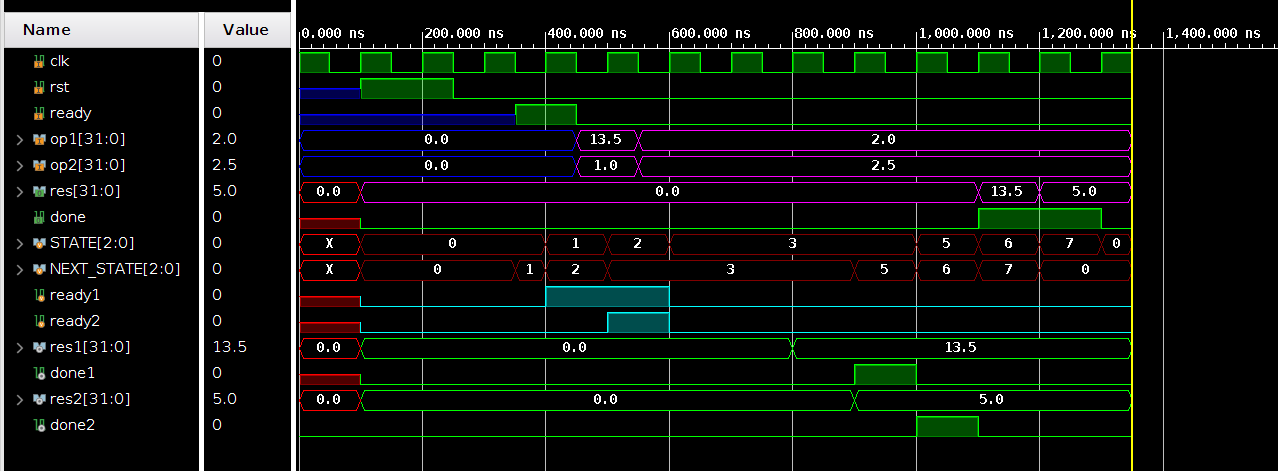
\includegraphics[width=\textwidth]{figures/sim_dm}
    \caption{Simulazione double\_multiplier in Verilog con script TCL}
    \label{fig:SIM_DM}
\end{figure*}

\begin{figure*}[bt]
    \centering
    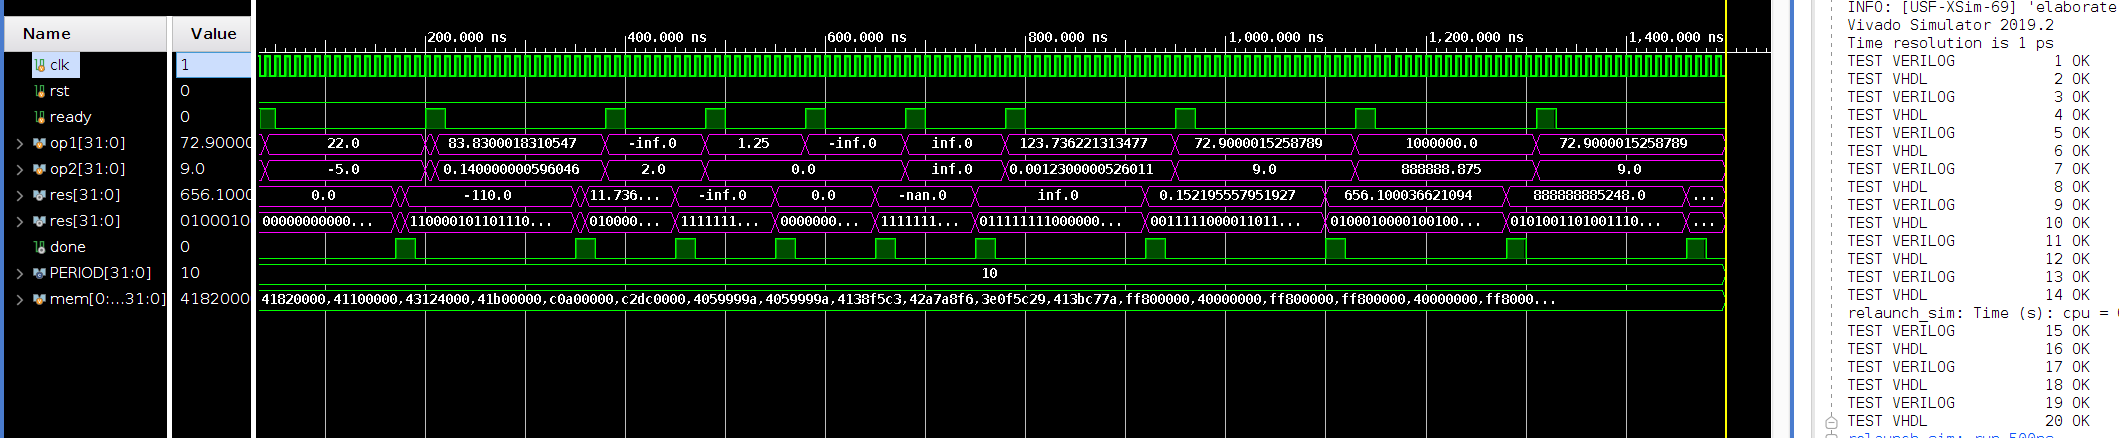
\includegraphics[width=\textwidth]{figures/sim_testbench}
    \caption{Simulazione double\_multiplier in Verilog con testbench}
    \label{fig:SIM_TESTBENCH}
\end{figure*}

\begin{figure*}[bt]
    \centering
    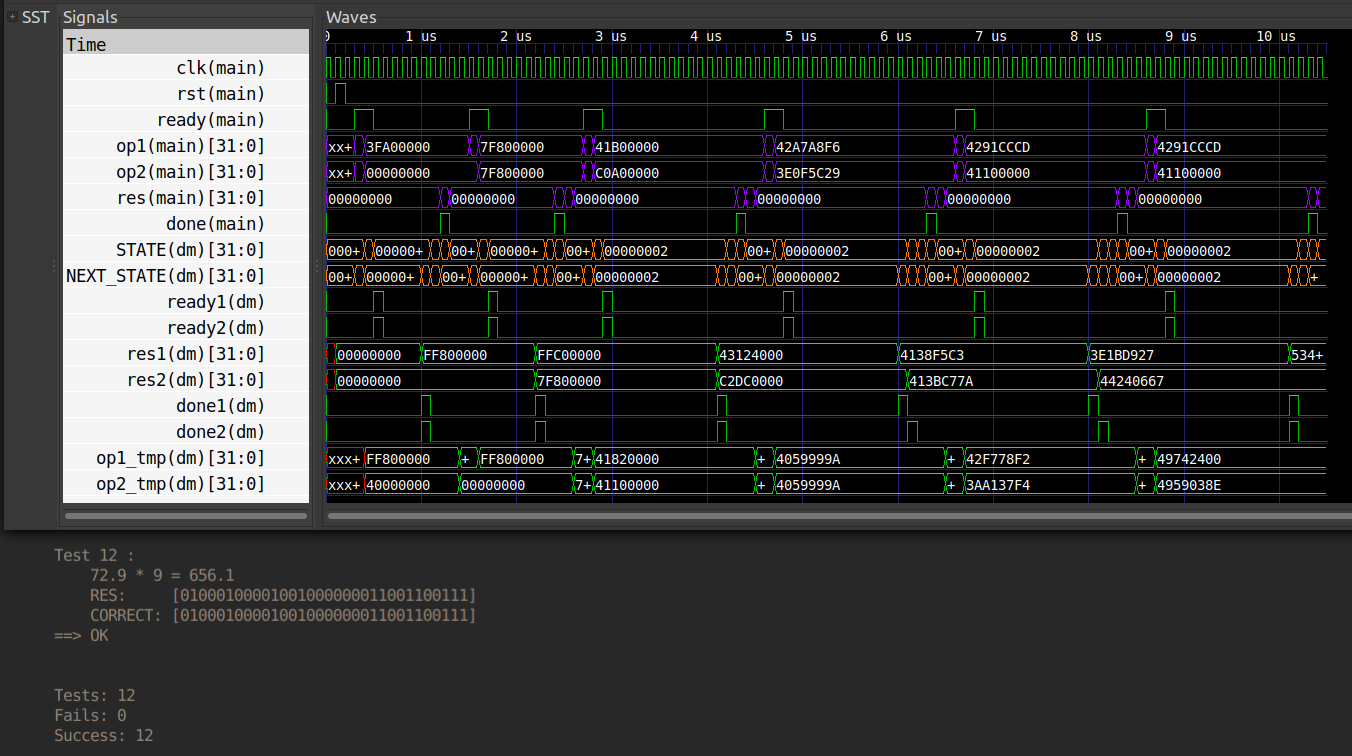
\includegraphics[width=\textwidth]{figures/sim_systemc_target}
    \caption{Simulazione double\_multiplier in SystemC con ``targeted test''}
    \label{fig:SIM_SC_TARGET}
\end{figure*}

\begin{figure*}[bt]
    \centering
    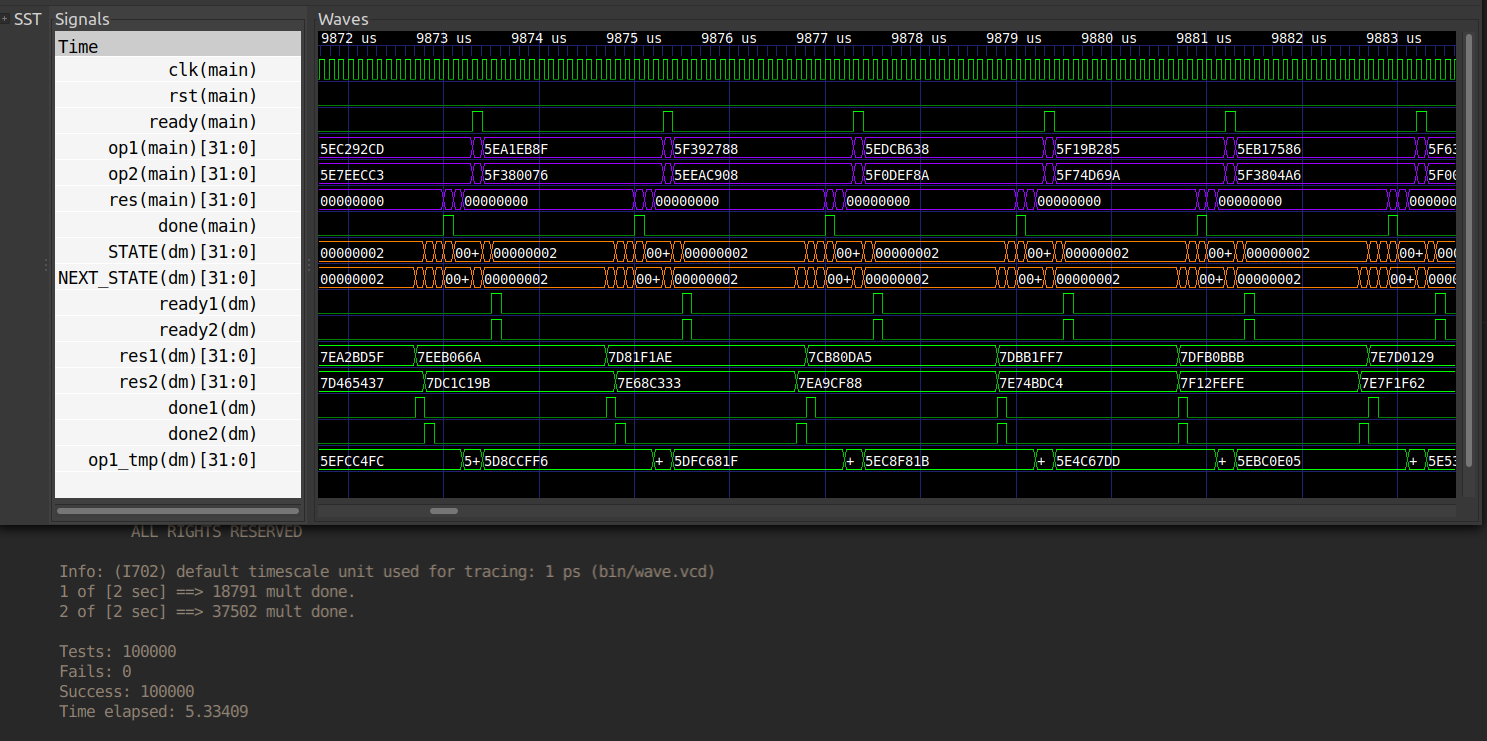
\includegraphics[width=\textwidth]{figures/sim_systemc_rnd}
    \caption{Simulazione double\_multiplier in SystemC con ``random test''}
    \label{fig:SIM_SC_RND}
\end{figure*}


\end{document}